\documentclass[tikz]{standalone}
\usepackage{pgfplots}
\pgfplotsset{compat=1.15}
\usepackage{mathrsfs}
\usetikzlibrary{arrows,calc}
\usepackage{tkz-euclide}
\pagestyle{empty}

\definecolor{AngleClr}{rgb}{0,0.39215686274509803,0}
\definecolor{ShapeClr}{rgb}{0.6,0.2,0}
\definecolor{BlueSqr}{RGB}{5,81,163}
\definecolor{RedSqr}{RGB}{0, 156, 0}

\begin{document}

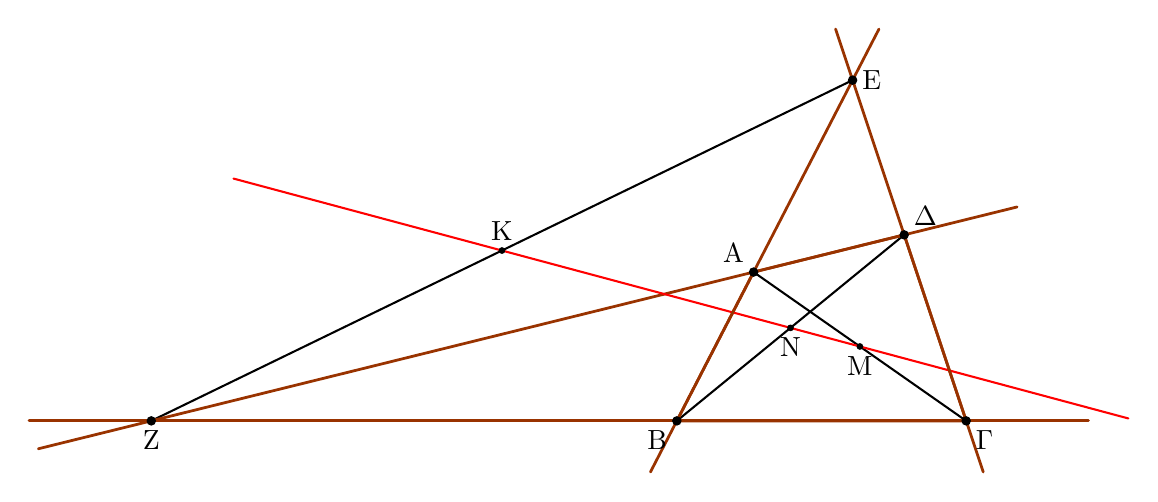
\begin{tikzpicture}[scale=.75]
\tkzSetUpLine[line width=1pt,color=black]
\tkzSetUpPoint[fill=black]

\tkzDefPoints{3.85/3.15/D,4.9/0/C,1.3/2.52/A,0/0/B}

\tkzInterLL(B,C)(A,D) \tkzGetPoint{Z}
\tkzInterLL(A,B)(C,D) \tkzGetPoint{E}

\tkzFillPolygon[fill=white](A,B,C,D)

\tkzDefMidPoint(A,C) \tkzGetPoint{M}
\tkzDefMidPoint(B,D) \tkzGetPoint{N}
\tkzDefMidPoint(E,Z) \tkzGetPoint{K}

% \tkzDefMidPoint(E,D) \tkzGetPoint{S}
% \tkzDefMidPoint(A,E) \tkzGetPoint{L}
% \tkzDefMidPoint(A,D) \tkzGetPoint{P}

\tkzDrawSegments[line width=0.75pt,color=black](A,C B,D E,Z) %  K,S N,S)
\tkzDrawSegments[line width=1pt,color=ShapeClr,add=0.15 and 0.15](C,Z C,E D,Z B,E)
\tkzDrawSegment[line width=0.75pt,color=red,add=0.75 and 0.75](M,K)


\tkzDrawPolygon[color=ShapeClr](A,B,C,D)
\tkzDrawPoints[size=3](A,B,C,D,E,Z)
\tkzDrawPoints[size=2](M,N,K)
\tkzLabelPoint[above left](A){$\rm A$}
\tkzLabelPoint[below left](B){$\rm B$}
\tkzLabelPoint[below right](C){$\rm \Gamma$}
\tkzLabelPoint[above right](D){$\rm \Delta$}

\node[below] at (M) {$\rm M$};
\node[below] at (N) {$\rm N$};
\tkzLabelPoint[above](K){$\rm K$}
\tkzLabelPoint[below](Z){$\rm Z$}
\tkzLabelPoint[right](E){$\rm E$}

% \tkzLabelPoint[above left](L){$\rm \Lambda$}
% \tkzLabelPoint[above right](S){$\rm \Sigma$}
% \tkzLabelPoint[below right](P){$\rm P$}



\end{tikzpicture}

\end{document}
